
\section{Solution: A lower scheduling class}\label{s:idle}

Rather than moving the LC workload up a class, we move the BE workload down.
Linux does not natively have a scheduling class below Normal, so we make use of
a scheduling policy that Linux has and already special cases in some
places.\hmng{this section is a weird middle between `design', which we don't
really have, and implementation}

\schedidle{} is a scheduling \textit{policy}. Policies are not full scheduling
classes, but allow for special casing within a scheduling class. The Normal
scheduling class supports two policies: \schednormal{}, the default, and
\schedidle{}. Because both policies are in the same class the scheduler for the
Normal class is in charge of both: it keeps the tasks of both policies on the
same runqueue, and they are all scheduled using the same algorithm. Thus,
\schedidle{} is in principle not very different from just being a low-weight
process: From the scheduler's perspective, \schedidle{} entities are just
entities with a predefined low weight (currently 3).\footnote{There is,
confusingly, also an Idle scheduling \textit{class}, but that not accessible to
userspace and exists solely to manage the core's transition in and out of being
actually idle (ie running nothing).}

The main way that the Normal scheduler special-cases \schedidle{} entities from
\schednormal{} entities is during wakeup: in a 2019 patch~\cite{TODO}, Linux
added a check where, when a \schednormal{} entity becomes newly runnable, if the
core where the entity is waking up is already running something in
\schednormal{}, it will look for other cores that might be currently running a
\schedidle{} entity, and migrates the new entity there.

In doing so, Linux created a half scheduling class. As discussed in
\autoref{ss:interface}, in order to fully isolate two groups of processes the
scheduler needs to try synchronize across cores at two points: entry and exit.
The described patch adds only the entry check.

\schedidle{} is additionally promising because it was extended to have cgroup
support recently\cite{TODO}: a whole groups' policy can be set to \schedidle{}
via the \cgroups{} interface.

\begin{figure}[t]
    \centering
    \begin{subfigure}[t]{0.49\columnwidth}
        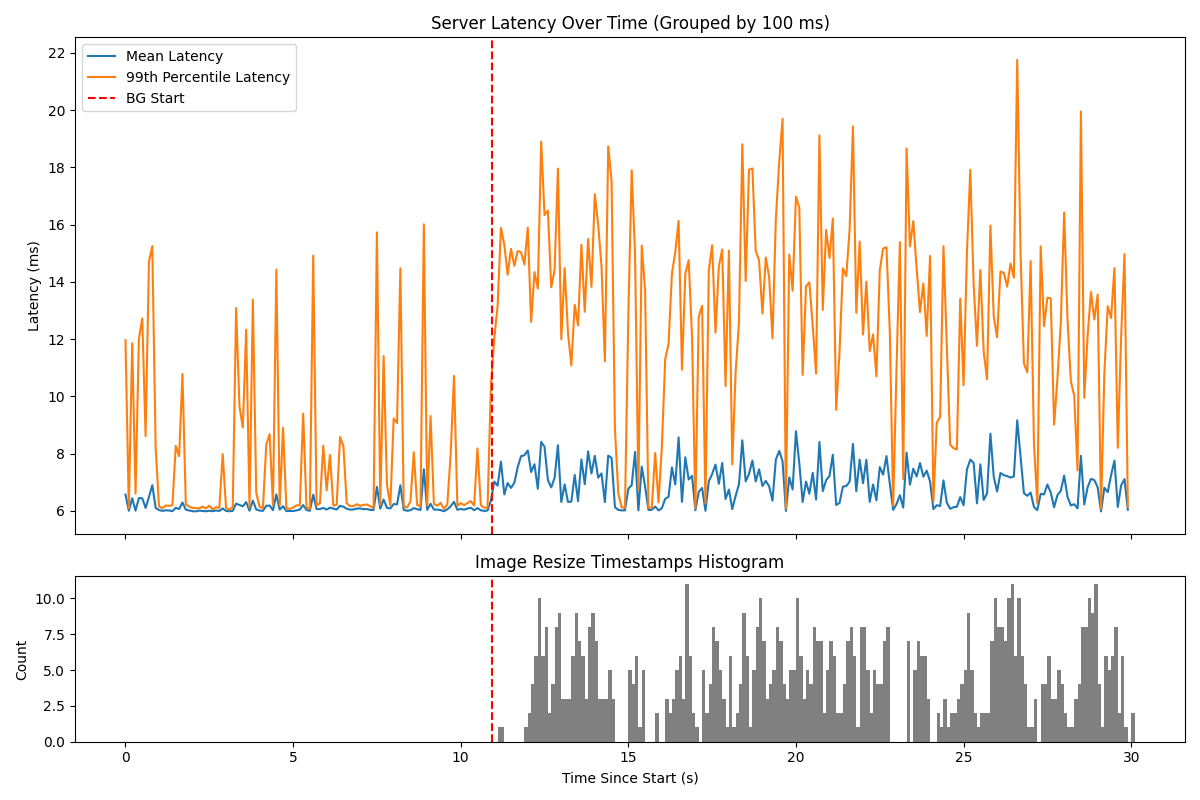
\includegraphics[width=\columnwidth]{graphs/unedited-idle-low-two.png}
        \caption{Low load}\label{fig:unedited-idle-low-two}
    \end{subfigure}
    \hspace{\fill}
    \begin{subfigure}[t]{0.49\columnwidth}
        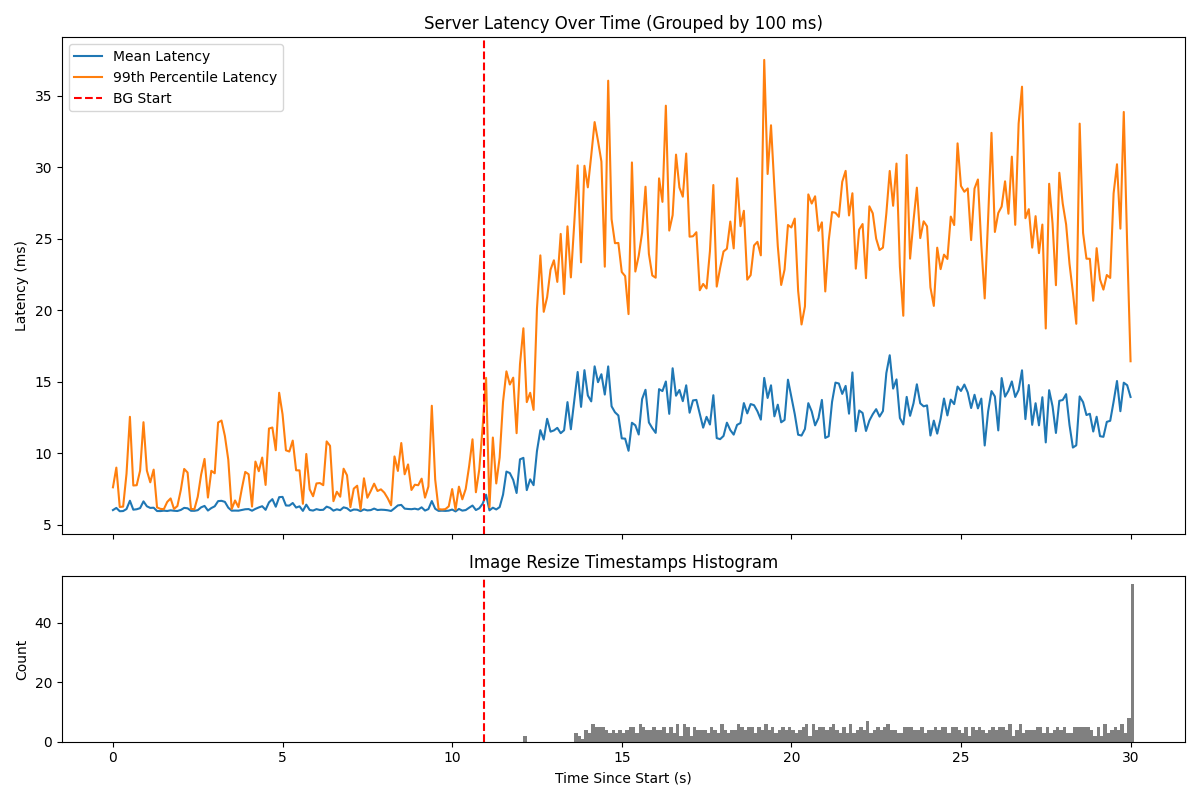
\includegraphics[width=\columnwidth]{graphs/unedited-idle-high-two.png}
        \caption{High load}\label{fig:unedited-idle-high-two}
    \end{subfigure}
    \vspace{4pt}
    \caption{using \schedidle{}}\label{fig:unedited-idle}
\end{figure}

And indeed, we find that when we use cgroups' new cpu.idle interface feature,
the latency impact of the BE tasks decreases, although it does not entirely drop
to what we saw with the Fifo class.\ \autoref{fig:unedited-idle} shows the
results, for the familiar settings of low and high load. The jump we see in the
mean latency has decreased from peaks as high as 13ms to around 7ms (even though
in principle they now have a higher weight).


